\documentclass{standalone}


\usepackage[europeanresistors,americaninductors]{circuitikz}

\begin{document}
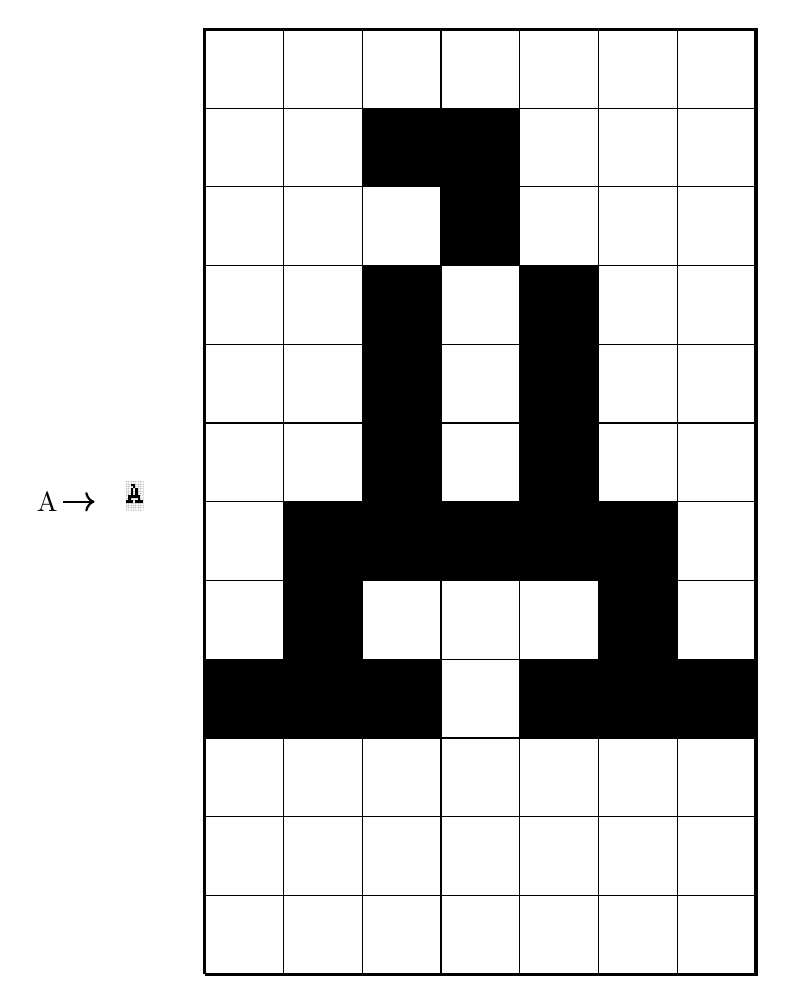
\begin{tikzpicture}
\node[anchor=center] at (-2, 6) {A};
\draw[thick, ->](-1.8,6)->(-1.4,6);
  \begin{scope}
%\draw [step=0.03,very thin] (-1, 5.9) grid (-0.79, 6.26);

\foreach \i in {-1,-0.97,...,-0.79}
{
	\draw [line width=0.001mm](\i, 5.9) -- (\i, 6.26);
}
\foreach \i in {5.9,5.93,...,6.26}
{
	\draw [line width=0.001mm](-1, \i) -- (-0.79, \i);
}

\fill [black] (-1, 5.99) rectangle (-0.91, 6.02);
\fill [black] (-0.88, 5.99) rectangle (-0.79, 6.02);
\fill [black] (-0.97, 6.02) rectangle (-0.94, 6.05);
\fill [black] (-0.85, 6.02) rectangle (-0.82, 6.05);
\fill [black] (-0.97, 6.05) rectangle (-0.82, 6.08);
\fill [black] (-0.94, 6.08) rectangle (-0.91, 6.17);
\fill [black] (-0.85, 6.08) rectangle (-0.88, 6.17);
\fill [black] (-0.88, 6.17) rectangle (-0.91, 6.20);
\fill [black] (-0.88, 6.20) rectangle (-0.94, 6.23);

\draw [fill=black] (4,3) rectangle (7,4);
\draw [fill=black] (1,4) rectangle (2,5);
\draw [fill=black] (5,4) rectangle (6,5);
\draw [fill=black] (1,5) rectangle (6,6);
\draw [fill=black] (2,6) rectangle (3,9);
\draw [fill=black] (4,6) rectangle (5,9);
\draw [fill=black] (3,9) rectangle (4,10);
\draw [fill=black] (2,10) rectangle (4,11);



\draw (0, 0) grid (7, 12);
\draw[very thick] (0,0) -- (7,0) -- (7,12) -- (0,12) -- (0,0);
\draw [fill=black] (0,3) rectangle (3,4);
\draw [fill=black] (4,3) rectangle (7,4);
\draw [fill=black] (1,4) rectangle (2,5);
\draw [fill=black] (5,4) rectangle (6,5);
\draw [fill=black] (1,5) rectangle (6,6);
\draw [fill=black] (2,6) rectangle (3,9);
\draw [fill=black] (4,6) rectangle (5,9);
\draw [fill=black] (3,9) rectangle (4,10);
\draw [fill=black] (2,10) rectangle (4,11);

%\node[anchor=center] at (3, -0.5) {Font size 12 Description 7 Pixel wide 12 High};
\end{scope}


\end{tikzpicture}
\end{document}
